\chapter{ Création de la base de données}
\vspace{5cm}
\large{Ce troisième chapitre st réservé à la création de la base de données.\\}


\newpage
\section{Shema de base de donnees}

\begin{minipage}{\linewidth}
	\makebox[\linewidth]{
		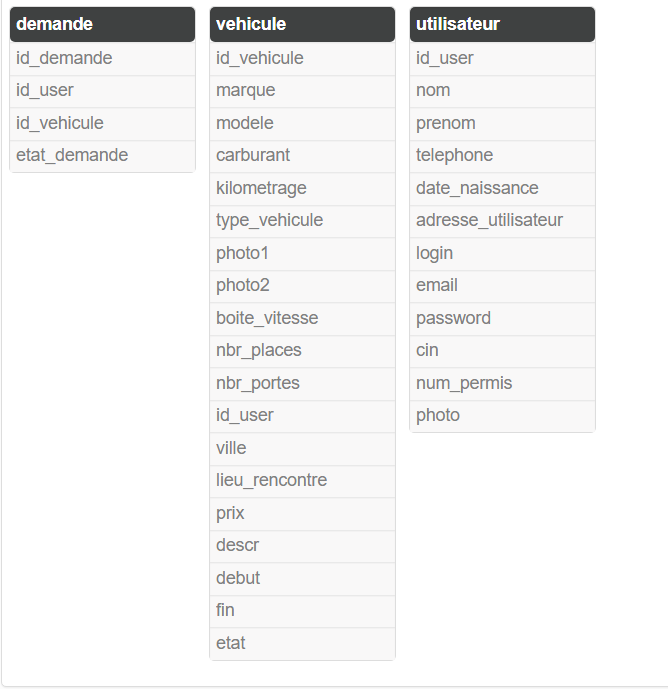
\includegraphics[keepaspectratio=true,scale=1.2]{data.PNG}}
	\captionof{figure}{shema de base de donnees}\label{f3}%    
\end{minipage}\\

\section{Signification de champs}
\begin{center}
\begin{table}[htp]

 \begin{tabular}{||c||  c||  c||  c||} 
 \hline
 Nom & ID & Type & Entite \\ [0.5ex] 
 \hline\hline
 identificateur de vehicule &  id\_vehicule & int & vehicule \\ 
 \hline
 Marque de vehicule & marque & varchar & vehicule \\
 \hline
 Modele de vehicule& modele & varchar & vehicule \\
 \hline
 
Type de carburant de vehicule& carburant & varchar & vehicule \\
 \hline
 
 kilometrage fait par le vehicule& kilometrage & int & vehicule \\
 \hline
  Type de vehicule& type\_vehicule & varchar & vehicule \\ 
 \hline
 photo1 de la vehicule& photo1 & varchar & vehicule \\
 \hline
 photo2 de la vehicule& photo2 & varchar & vehicule \\
 \hline
 Type de boite de vitesse& boite\_vitesse & varchar & vehicule \\
 \hline
 Nombre de places& nbr\_places & int & vehicule \\
 \hline
 Nombre de portes& nbr\_portes & int & vehicule \\
 \hline 
 ville & ville & varchar & vehicule \\
 \hline
 lieu de rencontre & lieu\_rencontre & varchar & vehicule \\
 \hline 
 Prix de l'offre& prix & int & vehicule \\
 \hline 
 Description de la vehicule& Descr & varchar & vehicule \\
 \hline 
 Date debut de disponibilite de vehicule& debut & date & vehicule \\
 \hline
 Date fin de disponibilite de vehicule&  fin & date & vehicule \\
 \hline 
 Etat de disponibilite de vehicule& etat & varchar & vehicule \\
 \hline
 Identificateur  de l'utilisater& id\_user & int & utilisateur \\
 \hline
 Nom  de l'utilisater& nom & varchar & utilisateur \\
 \hline
  Prénom  de l'utilisater& prenom & varchar & utilisateur \\
 \hline
 Date naissance  de l'utilisater & date\_naissance & date & utilisateur \\
 \hline
  Telephone  de l'utilisater& telephone & int & utilisateur \\
 \hline
 Adresse de l'utilisater & adresse\_utilisateur & varchar & utilisateur \\
 \hline 
 Login& login & varchar & utilisateur \\
 \hline 
 Email& email & varchar & utilisateur \\
 \hline 
 Mot de passe & password & varchar & utilisateur \\
 \hline 
 CIN & cin & varchar & utilisateur \\
 \hline 
  Numero de permis & num\_permis & varchar & utilisateur \\
 \hline 
  Photo de la vehicule& photo & varchar & utilisateur \\
 \hline 
  Identificateur de demande& id\_demande & int & demande \\
 \hline 
 Identificateur de utilisateur& id\_user & int & demande \\
 \hline 
  Identificateur de vehicule& id\_vehicule & int & demande \\
 \hline 
  Etat de traitement de demande & etat\_demande & varchar & demande \\
 \hline 


\end{tabular}
\caption{Signification de champs}
\end{table}
\end{center}
